% Shared standalone design for the editable figure reconstructions.
\documentclass[tikz,border=5pt,10pt]{standalone}
\usepackage[T1]{fontenc}
\usepackage[utf8]{inputenc}
\usepackage{newpxtext,newpxmath}
\usepackage[scaled=.94]{sourcesanspro}
\usepackage{pgfplots}
\pgfplotsset{compat=1.18}
\usetikzlibrary{arrows.meta,calc,positioning,decorations.pathreplacing,
  decorations.markings,patterns,matrix,shapes.geometric,fit,backgrounds,
  intersections,angles,quotes}
\definecolor{ink}{HTML}{203746}
\definecolor{accent}{HTML}{146C78}
\definecolor{muted}{HTML}{667780}
\definecolor{signalred}{HTML}{B94B44}
\color{ink}
\tikzset{>=Latex,line width=.8pt,
  every node/.style={font=\small},
  axis/.style={->,draw=muted,line width=.5pt},
  guide/.style={draw=muted,dashed,line width=.45pt},
  curve/.style={draw=accent,line width=1pt},
  marker/.style={circle,fill=accent,inner sep=1.5pt},
  labelbox/.style={fill=white,inner sep=2pt}}


\begin{document}

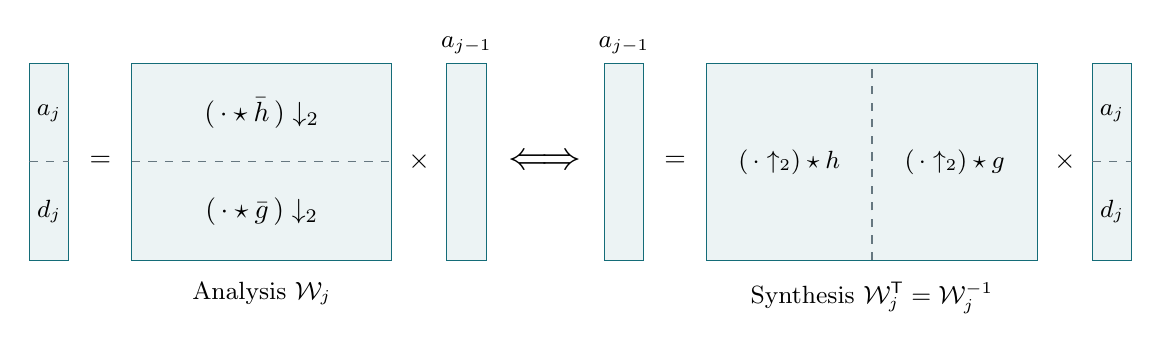
\begin{tikzpicture}[x=1cm,y=1cm]
\tikzset{block/.style={draw=accent,fill=accent!8},txt/.style={font=\normalsize}}
% Analysis: a stacked pair of half-height outputs and two operator rows.
\draw[block] (0,0) rectangle (.5,2.5);\draw[guide] (0,1.25)--(.5,1.25);
\node at (.25,1.87) {$a_j$};\node at (.25,.62) {$d_j$};\node[txt] at (.9,1.25) {$=$};
\draw[block] (1.3,0) rectangle (4.6,2.5);\draw[guide] (1.3,1.25)--(4.6,1.25);
\node[txt] at (2.95,1.87) {$(\,\cdot\star\bar h\,)\downarrow_2$};
\node[txt] at (2.95,.62) {$(\,\cdot\star\bar g\,)\downarrow_2$};
\node[txt] at (4.95,1.25) {$\times$};\draw[block] (5.3,0) rectangle (5.8,2.5);\node[above] at (5.55,2.5) {$a_{j-1}$};
\node[font=\Large] at (6.55,1.25) {$\Longleftrightarrow$};
% Synthesis: transpose block structure, horizontally concatenated operators.
\draw[block] (7.3,0) rectangle (7.8,2.5);\node[above] at (7.55,2.5) {$a_{j-1}$};\node[txt] at (8.2,1.25) {$=$};
\draw[block] (8.6,0) rectangle (12.8,2.5);\draw[guide] (10.7,0)--(10.7,2.5);
\node at (9.65,1.25) {$(\,\cdot\uparrow_2)\star h$};\node at (11.75,1.25) {$(\,\cdot\uparrow_2)\star g$};
\node[txt] at (13.15,1.25) {$\times$};\draw[block] (13.5,0) rectangle (14,2.5);\draw[guide] (13.5,1.25)--(14,1.25);
\node at (13.75,1.87) {$a_j$};\node at (13.75,.62) {$d_j$};
\node[below,align=center] at (2.95,-.15) {Analysis $\mathcal W_j$};\node[below] at (10.7,-.15) {Synthesis $\mathcal W_j^{\mathsf T}=\mathcal W_j^{-1}$};
\end{tikzpicture}

\end{document}
